\subsection{Gravitative Methode}

\begin{table}[H]
    \centering
    \caption{Benötigte Stromstärke, damit das Drehmoment des Magnetfeldes das der Gravitation ausgleicht.}
    \label{tab:grav}
    \begin{tblr}{
        colspec={S S},
        row{1}={guard, mode=math},
        \toprule
        d/\unit{\centi\meter}   &   I/\unit{\ampere}\\
        \midrule
        3.6  &   1.85   \\
        4.1  &   1.95   \\
        4.6  &   2.00   \\
        5.1  &   2.15   \\
        5.6  &   2.20   \\
        6.1  &   2.30   \\
        6.6  &   2.45   \\
        7.1  &   2.50   \\
        7.6  &   2.60   \\
        \bottomrule
        }
    \end{tblr}
\end{table}
\begin{figure}
    \centering
    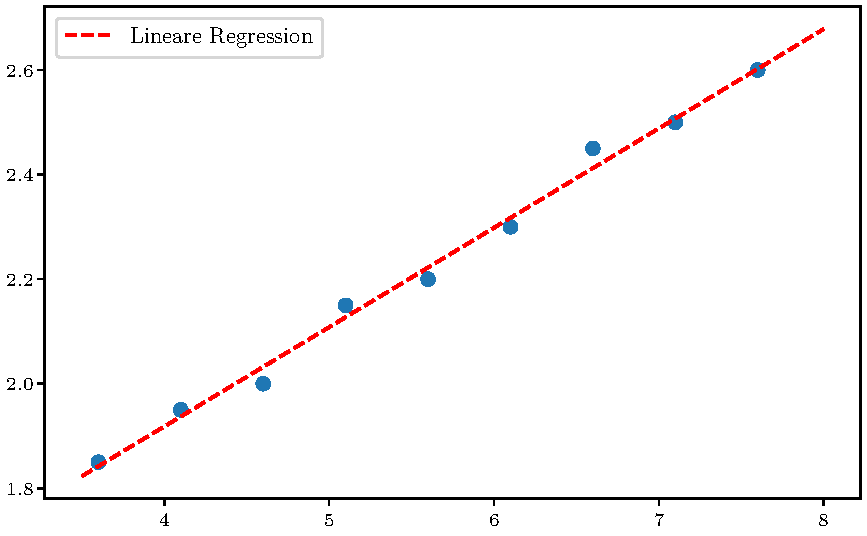
\includegraphics[width=\textwidth]{plot1.pdf}
    \label{fig:grav}
\end{figure}